\section{模拟方案}

Deidre H. 等人在论文\cite{hopkins_linear_2012} 中使用 NaI(Tl) 探测器探测经过准直器和 MCP-96 合金衰减后的多种能量的 $\gamma$ 的衰减情况。其歙砚设定如图\ref{fig:hopkins}。

\begin{figure}[H]
    \centering
    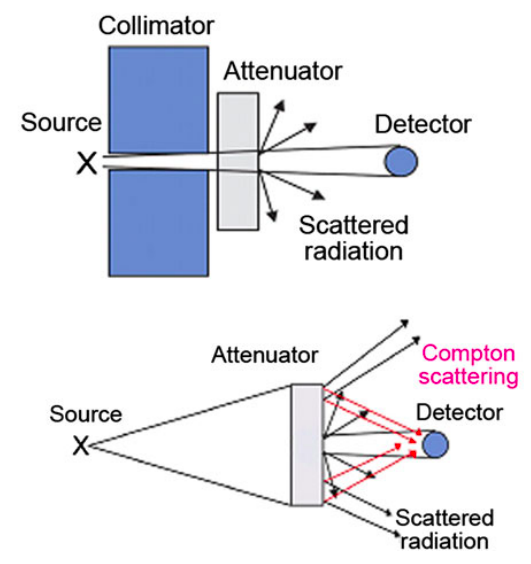
\includegraphics[width=\linewidth]{figures/hopkins.png}
    \caption{Deidre H. 论文中测量 MCP-96 特性的实验设计}
    \label{fig:hopkins}
\end{figure}

其中上图为设置了铅准直器和 MCP-96 合金的屏蔽体的实验设计,其中NaI(Tl)探测器晶体的截面积为 $5.08\times5.08\si{cm^2}$,MCP-96 衰减器的截面积为 $5\times5\si{cm^2}$,铅制准直器厚度为 $6\si{cm}$,中心圆孔的直径为 $1\si{cm}$。论文\cite{hopkins_linear_2012} 中使用 $^{60}Co,^{54}Mn,^{137}Cs$ 产生能量为 $0.662\si{MeV},0.835\si{MeV},1.17\si{MeV},1.33\si{MeV}$ 的 $\gamma$ 射线。实验中保持放射源与准直器的距离不变,准直器、MCP-96 衰减器、探测器的尺寸不变。只允许衰减器与探测器之间的距离 $d'$ 改变,从 $5\si{cm}$ 到 $15\si{cm}$ 采用每步 $1\si{cm}$ 变化;也允许 MCP-96 的厚度 $d$ 改变,从 $1\si{cm}$ 到 $4\si{cm}$ 采用每步 $1\si{cm}$ 变化。

在模拟中,放射源、准直器、衰减器和探测器的集合构造与图\ref{fig:hopkins}几乎相同,但使用点源代替论文\cite{hopkins_linear_2012}中的半径为 $1.27\si{cm}$ 的片状放射源。在模拟中,因为不受到天然放射源的能量只能取特定的分离值的限制,$\gamma$ 射线能量可以采取任意值。模拟中每种参数组合 $(d, E, d')$ 中进行 $10^5$ 次模拟,$\gamma$ 射线均采用各向同性发射,每次模拟均为单能射线。

通过准直器的加入,可以模拟窄束情况中,放射源直射入探测器的 $\gamma$ 光子个数,探测器所探测到的光子个数 $N_1$ 为公式\ref{eq:attenuation}中的 $N$。去掉准直器时,模拟宽束情况,此时探测器探测到的光子个数 $N_2$ 与上述加入准直器时探测器探测到的光子个数 $N_1$ 之比 $\frac{N_2}{N_1}$ 即为此时 MCP-96 的厚度 $d$ 和 $\gamma$ 射线能量 $E$ 的累计因子 $B(E, d)$。

图\ref{fig:sim}为屏蔽体厚度为 $4\si{cm}$ ,屏蔽体与探测器距离 $d'$ 为 $10\si{cm}$ 时的几何条件示意图,其中半透明圆盘为铅制准直器,红色色块为放射源,白色小长方体为 MCP-96 屏蔽体,黄色长方体为 NaI(Tl) 探测器。

\begin{figure}[H]
    \centering
    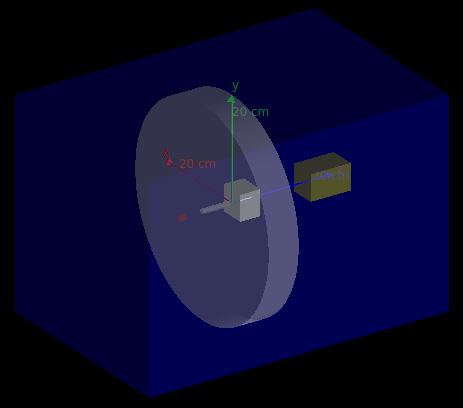
\includegraphics[width=\linewidth]{figures/sim.png}
    \caption{模拟 MCP-96 屏蔽体对 $\gamma$ 源的屏蔽效应的几何条件示意图}
    \label{fig:sim}
\end{figure}